\documentclass[12pt]{article}
\usepackage[utf8]{inputenc}

\usepackage{csquotes}
\usepackage{microtype}
\usepackage[english]{babel}
\usepackage{amsmath}

\usepackage[style=ieee, maxbibnames=5, backend=biber, url=false]{biblatex}
\addbibresource{MyLibrary.bib}
\usepackage{hyperref} % for hyperlinks
\usepackage[capitalise, noabbrev]{cleveref} % for \cref, MUST be loaded AFTER hyperref

\usepackage{booktabs} % midrule etc.
\usepackage{adjustbox} % for adjusting table width

% title and author and date
\title{MuZero for POMDPs by Recurrent Representation and Biasing Latent Space with Map Reconstruction}
\author{Jan Mrkos\\ AIC FEE CTU in Prague\\}
\date{\today}



\begin{document}
\maketitle
\section{Introduction}
% Option 2:

% RL in POMDPs is hard
Applying deep reinforcement learning (RL) algorithms to partially observable Markov decision processes (POMDPs) is difficult. 
One reason is poor sample efficiency, which is  already in issue in fully observable MDPs, but is exacerbated by partial observability. 
Second, principal reason, is state aliasing; where in POMDPs the same observations correspond to different environmental states.  

% Model-based RL helps
Model-based RL algorithms, such as MuZero~\cite{schrittwieserMasteringAtariGo2020}, are generally more sample efficient by constructing a model of the environment. 
This model is then used to supplement the agent's experience in the environment to plan actions. 
However, POMDPs pose a difficult problem for RL algorithms, as discovering the right model is much more challenging task in POMDPs than it is in MDPs. 

% Limitations of MuZero
Original MuZero algorithm is a model-based reinforcement learning algorithm that learns a model of the environment and uses it to plan and learn policies. 
It excels in deterministic, fully observable domains.
It also performs well with small amount of stochasticity, but the Stochastic MuZero~\cite{antonoglouPlanningStochasticEnvironments2021} algorithm obtains slightly better results~\cite{niuLightZeroUnifiedBenchmark2023}. 
This is also true in partially observable domains.
However, in general, MuZero, nor Stochastic MuZero are able to perform well in partially observable domains, as they lack mechanisms to propagate information collected from previous observations to the future decisions in the same episode. 

% MuZero and SLAMuZero
One option is to provide an algorithm with prior understanding of how the model should look like.
In this work, we are inspired by the SLAMuZero~\cite{fangSLAMuZeroPlanLearn2024} algorithm intended for the SLAM problem in robotics. 
In training, the SLAMuZero agent is provided with maps of the training environments, which provide an engineered abstraction for the agent to use to learn a model of the environment.
When the agent is deployed in a new environment, it uses the learned model to create a new map, based on the prior understanding of how the environmental model should look like.
However, the SLAMuZero algorithm is also missing a mechanism for keeping track of information collected in previous timesteps, which is essential for effective planning in partially observable domains.
% SLAMuZero is a variant of the MuZero algortihm that is able to reconstruct a map of an unknown environment while navigating through it.
% In SLAMuZero, the agent is provided with a number of training environments and their maps, which the agent uses to train a model that can create a map of a new environment.

% Hypothesis
We hypothesize that for efficiently extending the MuZero algorithms to partially observable domains, two things are needed. 
First, information collected in previous timesteps needs to propagate to the future decisions in the same episode. This can be achieved by using the previous latent space as additional input to the the representation network, which is the component responsibnle for encoding observations into the latent space.
However, this is not enough, as training such representation network is sample inefficient; with partial observations,  latent space may take a long time to learn a representation of the environment that is actually useful for planning, even though the actual environment model migh be simple.  
This can be helped by guiding the construction of the latent space in some way. 
We do this by having the model reconstruct a known, useful abstraction of the environment, such as map, from the latent states. 
This forces the latent space to encode information critical for planning in the environment, improving sample efficiency. 

In some domains, we have existing, readily available abstractions of the environment that we know to be useful for planning, such as maps in gridworld mazes. 
These abstractions, when used as a training target for the reconstruction from the latent state space, will force the agent to focus on learning the latent state space that encodes this information, and as a result, will converge faster. 
While using engineered abstractions goes against the idea of the bitter lesson, it is not necessary to use the abstractions for the whole training process, but only to shape the initial latent space.

In this work, we propose and investigate a novel architecture that extends MuZero. Our method incorporates an explicit memory mechanism to handle state aliasing and utilizes a map-reconstruction task to guide the latent space towards representations that are immediately useful for planning.
% We demonstrate that this combination leads to faster convergence and superior performance in challenging, partially observable environments.


\section{Literature Survey}

\subsection{Model-based Reinforcement Learning}
MuZero family of algorithms\cite{schrittwieserMasteringAtariGo2020,niuLightZeroUnifiedBenchmark2023} remains the state-of-the-art in model-based reinforcement learning. Model-based RL methods are distinguished from model-free RL by planning the effects of next actions with an internal model of the environment. 
MuZero algorothm learns this model from the agent's interactions with the environment, without assuming any prior knowledge. 

The original MuZero algorithm \cite{schrittwieserMasteringAtariGo2020} consists of three components built from neural networks, that are trained jointly. A representation network, which encodes observations into a latet state space, which forms the model of the environment. 
A dynamics network is trained to predict the next latent state given a latenr state and an action, allowing the agent to consider effect of different actions and to plan into the future. 
Finally, the prediction network takes the latent state and provides a distribution over actions that approximates the optimal policy, and the value of the latent state. In execution, the agent receives an observation from the environment and encodes it into a latent state using the representation network. 
Next, it uses the dynamics and value networks to perform Monte-Carlo tree search (MCTS) on the latent states, where the root of the tree holds the estimate of the best action to take in the next step. 
In training, the agent uses recorded episodes to update all three networks together. 

MuZero algorithm has been extended and improved in many different ways. 
For example, the Stochastic MuZero~\cite{antonoglouPlanningStochasticEnvironments2021} adds capability to model stochastic transitions, and demonstrates improved performance over the original MuZero algorithm. 
Other improvements include EfficientZero~\cite{yeMasteringAtariGames2021}, that among other improvements introduces consistency loss between the latent states from the representation network and latent states projected to the future with the dynamics network, which makes the method converge faster. LightZero framework~\cite{niuLightZeroUnifiedBenchmark2023} unifies multiple of these improvements and algorithms into a single package. 
However, these works focus squarely on fully observable domains, or domains that can be reasonably modelled as such. 

\subsection{Recurrent models and partial observability}
In MDPs, the agent can reason about the future based only on his known current state, which is what MuZero does. However, partial observable MDPs give agent limited observations about his state, and require the agent to build a distribution over the possible states he might be in, the belief, based on the history of all previous observations. Example of a POMDP problem is Simultaneous Localization and Mapping (SLAM) problem in robotics, assuming limited robot sensors. 

SLAMuZero~\cite{fangSLAMuZeroPlanLearn2024} is a recent attempt at applying MuZero to SLAM. 
SLAMuZero builds on prior work by~\textcite{chaplotLearningExploreUsing2020}, however, it ignores the additive construction of the map based on the sequence of observations, which is a crucial aspect of that work. 
Instead, SLAMuZero generates full map estimates from every observation, with no mechanism to enforce consistency and stabiility of the generated map. 

The mechanism of constructing the map from~\textcite{chaplotLearningExploreUsing2020} relies on using the partial map and position estimate from the previous timestep with the new observation to construct a slighly larger map and position estimate in it for use in the next timestep. 
This mechanism can be replicated in MuZero by using the previous latent state as an additional input to the representation network, using recurrent neural network.
Such mechanism is crucial for dealing with partial observability, as it allows the agent to compress history of observations into a belief about the environment and agent's position in it. 

Recurrent latent-state model is foundation of the Dreamer algorithms~\cite{hafnerMasteringDiverseDomains2024} using the Recurrent State Space Model (RSSM)~\cite{hafnerLearningLatentDynamics2019}. The RSSM is a recurrent model for encoding POMDP observations into a latent state space. It splits the latent state into two parts, a deterministic part, acting as a memory, which authors argue is essential for the agent to remember facts reliably over time, and a stochastic part, which is required to express the uncertainty about the environment and is crucial for the agent to learn at all. This is similar to how~\textcite{chaplotLearningExploreUsing2020} constructs a deterministic map of the observations, together with a second channel that encodes the uncertainty about the agent's position in the map.
Unlike our approach, the RSSM relies on rich, informative observations, whereas we are interested in low-dimensional, aliased observations. Additionally, the dreamer algorithms use RSSM to generate sequences of states that are used to train the actor networks, whereas we want to use the latent states to plan on.

% \subsection{Auxiliary loss for representation learning}
% Using the map reconstruction task as an auxiliary loss is a form of inductive bias. \textcite{fangSLAMuZeroPlanLearn2024} uses the known maps of the training environments to train the agent for faster exploration in unknown environments. 

\section{MuZeroRec and MuZeroRecMap algorithms}
We propose two modifications of the MuZero algorithm.
The following descriptions use the notation from the original MuZero paper~\cite{schrittwieserMasteringAtariGo2020}.

\subsection{MuZeroRec: Recurrent Representation}

The first variant, MuZeroRec, modifies the standard MuZero to handle partial observability by introducing recurrence into the representation process.
In the original MuZero, the representation network $h$ maps the current observation $o_t$ to a latent state $s_t$, i.e., $s_t = h(o_t)$.
This is memoryless and insufficient for POMDPs where the history of observations is required to reason about the belief.

In MuZeroRec, we modify the representation network to be recurrent.
The new network, $h_{\text{rec}}$, takes as input both the current observation $o_t$ and the latent state from the previous timestep, $s_{t-1}$.
The new latent state is then computed as:
$$s_t = h_{\text{rec}}(o_t, s_{t-1})$$
This allows the model to integrate information over time, enabling the latent state $s_t$ to represent a beliefs. In the initial experiments, we use MLP as the representation network, but RSSM may be useful here. 
The dynamics and prediction networks remain unchanged, operating on this more informed latent state.

The new structure of the representation network means that the MuZeroRec algorithm must be trained on full episodes, rather than on individual transitions. 

\subsection{MuZeroRecMap: Guiding Representation with Map Reconstruction}

The MuZeroRecMap algorithm builds upon MuZeroRec by introducing an auxiliary task to bias latent space. In addition to the recurrent representation network, we add a new component: a \textbf{decoder network}, denoted by $d$.

The function of the decoder is to reconstruct a 2D, 2-channel map of the environment from any given latent state $s_t$.. The first channel is the map,  $\hat{m}_t$, and the second channel is the estimate of agents position, $\hat{l}_t$. Specifically, the output of the decoder $\hat{m}_t, \hat{l}_t = d(s_t)$ is a grid where each cell contains possible tile types (e.g., empty, wall, goal) in the first channel, and the probability distribution over the tiles in the second channel, which signifies the agents belief about the agent's current position in the map. The belief about the agent's orientation can be encoded into the map as well, or provided as an additional output from the decoder. 

To train this decoder, we add an auxiliary loss term to MuZero's main training objective. This map reconstruction loss, $\mathcal{L}_{\text{map}}$, measures the difference between the reconstructed map $\hat{m}_t$ and the ground-truth map $m_{\text{true}}$, and $\mathcal{L}_{\text{pose}}$ measure difference between estimated location and actual, known location if moving from a known position, or a distribution over possible states after teleportation. 
The total loss for the agent is a weighted sum of the original MuZero losses (for policy, value, etc.) and this new map reconstruction loss. The map loss should provide a strong inductive bias that will force the latent space to focus on spatial information, which we hypothesize will accelerate learning and improve planning.

\section{Hypothesis}
The main hypothesis for this work is that that we can improve the performance of the MuZero algorithm in partially observable domains by recurrent representation network, and by guiding the construction of the latent space with a prior knowledge of how the environment abstraction looks like.

We have three main hypothesis:
\begin{itemize}
    \item \textbf{H1: Recurrent Representation - MuZeroRec} Making the representation network recurrent will allow the agent to keep track of the information collected in previous timesteps, allowing the MuZero agent to operate in partially observable domains. This is required for the agent to be able to compress observations into beliefs about the environment, which is essential for effective planning in partially observable domains.
    \item \textbf{H2: Map Abstraction - MuZeroRecMap} The "map reconstruction" task will guide the latent space towards representations that are useful for planning, improving sample efficiency.
    \item \textbf{H3: Bias} The combination of recurrent representation network and map reconstruction task leads to faster convergence and superior performance in in partially observable environments. However, assuming that the map is not an optimal abstraction, the map reconstruction loss biases the latent space. 
\end{itemize}

Baseline for the experiments is the original MuZero algorithm. For testing H1, we will use the MuZero algorithm with recurrent representation network, the MuZeroRec algorithm. For testing H2, we will use the MuZeroRec algorithm with the map reconstruction task, the MuZeroRecMap algorithm. For testing H3, we will compare the performance of the MuZeroRecMap algorithm with the MuZeroRec algorithm. 

For H1, we want to show improved performance in terms of collected reward of the MuZero and MuZeroRec algorithms. This is because training the recurrent representation need not be more efficient, and will require training on full epiosodes instead of transitions. As such, it would be unfair to compare the sample efficiency to the baseline. 

For H2, we want to show that the MuZeroRecMap algorithm is more sample efficient that the MuZeroRec algorithm, so we will be looking at the number of episodes needed to reach the same performance level.
Note, that it would be difficult to test H2 by applying map reconstruction to original MuZero, as is done by~\cite{fangSLAMuZeroPlanLearn2024}; in evaluation, we would be asking the agent to construct the whole map of the environment from each observation, without the ability to use the previous observations. 

However, we assume that introducing the map reconstruction loss restrains the MuZeroRec algortihm from finding the best possible abstraction. 
Therefore to test H3, we will select domain sizes where we can run MuZeroRec and MuZeroRecMap to convergence, and compare their performance.  
We expect the MuZeroRecMap algorithm to achieve good performance faster, but MuZeroRec should eventually outperform it. 
By exploring the tradeoff between the performance and the sample efficiency, we can then propose a method that biases the latent states in the initial stages of training, and turns of the map reconstruction loss later.

The map reconstruction network can also be useful to explore the structure of the latent space in novel environments, and to understand how the agent perceives the environment.

The experiment environment will be gridworld mazes for simplicity and because they are standard problem in RL literature and have easily defined maps that can be used as the target for the map reconstruction task.

\section{Experimental setup}
Our gridworld mazes will be based on the standard minigrid library, part of the OpenAI Gym. However, we will need to modify the mazes to fit our needs. 
What we need is following:

\begin{itemize}
    \item Partial observability: the agent will only see small part of the world.
    \item Useful mapping: we want the agent to learn the map of the environment, and we want the agent to have the opportunity to improve his performance by using the map.
    \item Stochasticity: we want the agent to be able to implicityly learn belief over the map. 
\end{itemize}

These requirements lead us to the folowing design of the training and evaluation environments. The maze contains wall cells, empty cells, single goal cell and an agent. The agent starts in predetermined position in randomly selected maze, with single goal tile positionws in the maze. Reaching the goal tile gives the agent positive reward, every step incurs a small negative reward. To force partial observability, the viewport of the agent is limited to a small area in front of the agent, 3x3 tiles, with the agent centered on one side of the viewport. This means that observations in different states will be aliased. 

To make exploaration of the map useful, wthe goal cell is not a terminal state, instead, we terminate episodes after predetermined number of steps, and we teleport the agent to a random position in the maze after reaching the goal tile. This also introduces stochastic transitions to the model, and the agent needs to deal with the uncertainty of its position in the maze after each teleportation. It can use its aliased observations to orient itself in the maze, and then use the map to plan its route to the goal tile. To reinforce the map use even more strongly, we have a deterministic movement and observatioon model with no stochasticity. In training, the agent will be trained on a set of randomly generated mazes, with previously unseen mazes used for evaluation.

\section{Implementation and dead ends}

\begin{table}
    \centering
    \begin{adjustbox}{width=\textwidth}
    \begin{tabular}{lllrrlp{6cm}l}
        \toprule
        Package & Language &           Author &  Contr. &  Stars & Last Update &                                                                                                                                                                                                                                                                                    Description &  Libraries \\
        \midrule
        \href{https://github.com/opendilab/LightZero}{LightZero} &   Python &        opendilab &            23 &   1300 &      2/2025 &                                                                                                                                                                                                                 Implementation of multiple MuZero algorithms in PyTorch. Also includes UniZero &    Pytorch \\
        \href{https://github.com/werner-duvaud/muzero-general}{muzero-general} &   Python &    werner-duvaud &            16 &   2600 &        2022 &                                                                                                                                                                                                                                                                 Open reimplementaion of MuZero &    Pytorch \\
        \href{https://github.com/google-deepmind/mctx}{mctx} &   Python &  google-deepmind &            10 &   2400 &     12/2024 &                                                                                                                                                                                                                                                       DeepMind implementation of MuZero in Jax &        Jax \\
        \href{https://github.com/kaesve/muzero}{muzero} &   Python &           kaesve &             3 &    156 &        2021 & from \href{https://arxiv.org/abs/2102.12924}{arxiv}, implementation extends AlphaZero to work with singleplayer domains, like its successor MuZero, and compares the two. & Tensorflow \\
        \href{https://github.com/YeWR/EfficientZero}{EfficientZero} &   Python &             YeWR &             2 &    883 &        2022 &                                                                                                                                                                                                                                                          From “Efficient Zero” Neurips paper &    Pytorch \\
        \href{https://github.com/johan-gras/MuZero}{MuZero} &   Python &       johan-gras &             1 &    207 &        2019 &                                                                                                                                                                                                                                                                                             &         \\
        \href{https://github.com/chiamp/sigmazero}{sigmazero} &   Python &           chiamp &             1 &      5 &      4/2024 &                                                                                                                                                                                                                              Seems to be and independent implementation of stochastic MuZero & Tensorflow \\
        \href{https://github.com/jonathan-laurent/AlphaZero.jl}{AlphaZero.jl} &    Julia & jonathan-laurent &            10 &   1300 &     12/2024 &                                                                                                                                                                                                                                                              AlphaZero implementation in Julia &         \\
        \href{https://github.com/deveshjawla/MuZero.jl}{MuZero.jl} &    Julia &      deveshjawla &             2 &      8 &        2021 &                                                                                                                                                                                                                                                                                MuZero in Julia &         \\
        \bottomrule
    \end{tabular}
    \end{adjustbox}
    \caption{Overview of AlphaZero derivatives implementations in Python and Julia.}
\end{table}
    
Based on my survey of RL libraries in Python and Julia, where I structured libraries by their relevance, latest github activity, number of stars and contributors, I have first explored the option of replicating experiments from the SLAMuZero paper~\cite{fangSLAMuZeroPlanLearn2024}. 

This seemed feasible at the first sight, SLAMuZero was presented at a conference recently and had code available on GitHub\footnote{\url{https://github.com/bwfbowen/SLAMuZero}}, and its main RL dependency was on a older fork of a DeepMind acme\footnote{\url{https://github.com/google-deepmind/acme}} library, which appeared to be actively maintained. Even though the SLAMuZero package itself has multiple complex dependencies, and the setup is not well documented, the dependencies appeared actively maintained. After many attempts and alot of guesswork I managed to install the package, together with all its dependencies and datasets. However, I was not able to get the code running, I assumed it was because of incorrectly set-up FacebookResearch Habitat environment\footnote{\url{https://github.com/facebookresearch/habitat-lab}} that was not compatible with SLAMuZero. I decided that trying to setup Habitat correctly was not worth the effort, as I did not plan on using the Habitat environment for my experiments.

Instead, I have decided to replace the Habitat environment with the minigrid\footnote{\url{https://minigrid.farama.org/}} environment, which is a standard RL environment for gridworld mazes in OpenAI Gym. As such, my plan was to reimplement SLAMuZero code with latest version of the DeepMind acme library, as SLAMuZero implementation was based on a fork of the outdated variant of the acme library. However, it turned out that while there is activity in the acme library repository, it is from github bots, and the library is not maintained and seemingly impossible to install with unsolvable dependencies\footnote{\url{https://github.com/google-deepmind/acme/issues/321}} that I also ran into.

At that point, I revisited the survey of implementations of AlphaZero derivatives, and found that LightZero package\footnote{\url{https://github.com/opendilab/LightZero}} is actively maintained, well documented and implements MuZero, along with other variants, and includes examples of how to use MuZero with the minigrid environment. Description of how to install and setup LightZero with custom minigrid environments are in the pZero package\footnote{\url{https://github.com/aicenter/pZero}} README.md file.

\section{Results}
I obtained useful results only for the MuZero algorithm, as the MuZeroRec did not seem to learn in my attempts at recurrent representation network. Figure~\ref{fig:MuZero_learning} shows the average evaluation reward of the vanilla MuZero algorithm. 

\begin{figure}[h!]
  \centering
  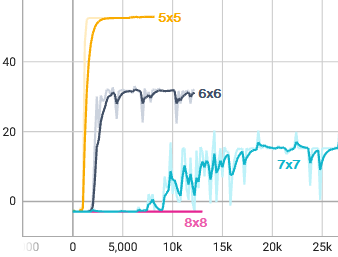
\includegraphics[width=0.4\textwidth]{MuZero_learning.png}
  \caption{Avarage evaluation reward of the vanilla MuZero algorithm during training in mazes of different sizes. While in 5x5 maze the agent qickly converges to a good policy, in 8x8 maze, the agent fails to learn any useful policy.}
  \label{fig:MuZero_learning}
\end{figure}

\end{document}